\documentclass[twocol]{ametsoc}
% \documentclass[]{ametsoc}
\usepackage[]{graphicx}
\usepackage{alltt}
\usepackage{siunitx}
%
%==============================================================================
\journal{jcli}

%
%==============================================================================
\bibpunct{(}{)}{;}{a}{}{,}

\title{Effects of Natural Variability of Seawater Temperature, Time Series Length, Decadal Trend and Instrument Precision on the Ability to Detect Temperature Trends}

\authors{Robert Schlegel\correspondingauthor{Robert Schlegel, Department of Biodiversity and Conservation Biology, University of the Western Cape, Bellville, Republic of South Africa.}
 and Albertus Smit}

\affiliation{Department of Biodiversity and Conservation Biology, University of the Western Cape, Bellville, Republic of South Africa}

\email{3503570@myuwc.ac.za}

%
%==============================================================================
\abstract{In South Africa 129 \emph{in situ} temperature time series of 1 to 43 years are used for investigations of the thermal characteristics of coastal seawater. They are comprised of temperature recordings at precisions ranging from \SIrange{0.5}{0.001}{\degreeCelsius} and collected with handheld thermometers or underwater temperature recorders (UTRs). Using the naturally occurring range of seasonal signals, variability and temperature trends for 84 of these time series, the length, decadal trend and data precision of each time series were systematically varied before fitting generalized least squares (GLS) models to study the effect these variables have on trend detection. We determined that the variables contributing most to accurate trend detection in decreasing order are: the length of the time series, the decadal trend, variance, amount of missing data and the precision of the measurements. We found that time series at least 20 years in length may be used tentatively for climate change research, but that time series \textgreater 30 years in length are preferable. The implication is that long-running thermometer time series in this dataset, and others around the world, are more useful for decadal scale climate change studies than the shorter, more precise UTR time series. It is important to note that due to the nature of the dataset used in this study, instrument drift was not able to be quantified.}

% AJS: At the same length, which is most useful: thermometer or UTR recordings?
% RWS: Given everything I've learned of instrument precision and the results of these analyses, I would say they are the same. I was going to say so in the abstract but decided against it. I need to perform an investigation into this by comparing closeness of fit to DT_model and DT with varying length against the different types. I think thermo's may actually be better....

% RWS: The abstract may need to be changed as we have shown that 0.5C precision may actually have a greater effect on the accuracy of a time series than variance.

% \emph{We need to say something at the end about things we did not study, which may be more important i.t.o. trend detection -- instrumental drift. There is also the aspect of accuracy that can/should be mentioned, and although (given a stable instrument without drift) can yield reliable, useful and precise trend estimates, can nevertheless be off in regards to know the real temperature.}
% RWS: Added a sentence at the end.

%==============================================================================
\begin{document}

\maketitle

\section{Introduction}
The roughly 3,000 km of South Africa's coastline is bordered by the Benguela and Agulhas currents \citep[e.g.][]{Roberts2005,Hutchings2009}, which, in combination with other nearshore processes, affect the country's marine coastal ecosystems \citep{Santos2012a}. A thorough understanding of these coastal processes is provided by several physical variables, of which temperature is one of the main determinants \citep[e.g.][]{Blanchette2008, Tittensor2010, Couce2012}. In order to ensure a true representation of organisms' biological thermal limits, nearshore temperatures must be accurately recorded and monitored. Some sources warn of the pitfalls in doing so \emph{RWS: Add references here showing which sources say using SST for the coast is inappropriate}, and a study by \citet{Smit2013} showed that SST data have a warm bias as large as \SI{6}{\degreeCelsius} when compared to coastal \emph{in situ} data. Nevertheless, a widespread approach in coastal ecological research is to use satellite and/or model-generated temperature data as representation of the sea surface temperature (SST) along coastlines \citep[e.g.][]{Blanchette2008, Broitman2008a, Tyberghein2012}, because apparently the dangers of applying gridded SSTs to the coast are not widely known or in many places in the world there simply are no suitable \emph{in situ} coastal temperature time series available. It is for this reason that we strongly recommended the use of \emph{in situ} data to support research conducted within 400 m from the shoreline.

Where records of \emph{in situ} coastal seawater temperature do exist, the reliability of many of these datasets that could be used in place of the remotely-sensed SST data remains to be verified. Users of SST data benefit from it being refined through a number of well documented validation and quality control processes \citep[e.g.][]{Reynolds1994, Brown1999, Martin2012}, whereas the standards and methods with which local \emph{in situ} data from a single dataset are collected and refined may differ greatly. For example, there are currently seven organizations and/or governmental departments (hereafter referred to as bodies) contributing coastal seawater temperature data to the South African Coastal Temperature Network (SACTN). These bodies use different methods and instruments to collect their data as no national standard has been set. One consequence of this methodological disparity is that two thirds of the data were sampled with hand-held thermometers that are manually recorded at a data precision of \SI{0.5}{\degreeCelsius}, as opposed to the current generation of Underwater Temperature Recorders (UTRs) with an instrument precision of down to \SI{0.001}{\degreeCelsius}. If these \emph{in situ} data are to be used together \emph{in lieu} of the satellite-based SST data, it is important that the characteristics of the contributing data sources are understood in terms of their ability to yield useful, reliable and accurate long-term measurements for use in climate change studies.

This prompted us to examine the 129 \emph{in situ} time series that comprise the SACTN. The range of measurement precisions and statistical characteristics of this dataset were used to guide a series of enquiry-driven analyses into the suitability of the time series to yield statistically significant and accurate assessments of decadal temperature change. The length, decadal trend and data precision of each time series were adjusted in a systematic manner, and forms the core of our analyses. Our aim was to assess the effect that each of these variables has on the ability of a model to produce a robust estimate of time series decadal trend. The effect gaps in the time series may have on the fitting of models was also investigated as many of the time series used here have some missing data scattered throughout, which is unavoidable for a 20+ year time series that is sampled by hand by a single technician at each site.

The study provides a better understanding of some of the determinants of a time series that are influential in the detection success of decadal trends in coastal ocean temperature time series.

\section{Methods}

\subsection{Data Sources}
Our study lies within the political borders of South Africa's coastline. The location of each point of collection appears in Figure \ref{figure01}. Of the 129 time series used, 43 are recorded with UTRs and the other 86 with hand-held mercury thermometers. The oldest currently running time series began on January 1st, 1972; there are 11 total time series that started in the 70s, 53 more started in the 80s, 34 began in the 90s, 18 in the 00s and 13 in the current decade.

The data are collected using two different methods and a variety of instruments. Hand-held mercury thermometers (which are being phased out in favor of alcohol thermometers or electronic instruments) are used in some instances at the shoreline, and represent seawater temperatures at the surface. At other places, predominantly along the country's east coast, data are collected with glass thermometers from small boats at the location of shark nets along the coast \citep{Cliff1988}. Whereas both types of thermometers allow for a measurement precision of \SI{0.1}{\degreeCelsius}, the recordings are written down at a precision of \SI{0.5}{\degreeCelsius}. Data at other localities are collected using delayed-mode instruments that are permanently moored shallower than 10 m, but generally very close to the surface below the low-water spring tide level.

Over the last 40+ years the electronic instruments used to measure coastal seawater temperatures have changed and improved. The previous standard was the Onset Hobo UTR with a thermal precision of \SI{0.01}{\degreeCelsius}. The new standard currently being phased in is the Starmon Mini UTR. These devices have a maximum thermal precision of \SI[separate-uncertainty = true, multi-part-units = repeat]{0.001(25)}{\degreeCelsius} (http://www.star-oddi.com/). Of the 43 UTR time series in this dataset, 30 were recorded at a precision of \SI{0.001}{\degreeCelsius} for their entirety, five UTR time series include older data that were recorded at a precision of \SI{0.01}{\degreeCelsius} or \SI{0.1}{\degreeCelsius} and so have been rounded down to match this level of precision. Eight additional UTR time series have older data that were recorded at a precision of \SI{0.1}{\degreeCelsius}.

The thermometer data are recorded manually and saved in an aggregated location at the head offices of the collecting bodies. UTRs are installed and maintained by divers and data are retrieved at least once annually. These data are digital and are downloaded to a hard drive at the respective head offices of the collecting bodies.

\subsection{Data Management}
Each of the seven bodies contributing data to this study have their own method of data formatting. Steps are being taken towards a national standard as we move towards replacing all the thermometer recordings with UTR devices; however, as of the writing of this article, one does not yet exist. Data from each organization were formatted to a project-wide comma-separated values (CSV) format with consistent column headers before any statistical analyses were performed. This allowed for the same methodology to be used across the entire dataset, ensuring consistent analysis. Before analysing the data they were scanned for any values above \SI{35}{\degreeCelsius} or below \SI{0}{\degreeCelsius}. These data points were changed to \texttt{NA}, meaning `not available', before including them in the SACTN dataset.

All analyses and data management performed in this paper were conducted with R version 3.3.1 (2016-06-21) \citep{R}. The script and data used to conduct the analyses and create the tables and figures in this paper may be found at https://github.com/schrob040/Trend\_Analysis.

Any time series with a temporal precision greater than one day were averaged into daily values before being aggregated into the SACTN. A series of additional checks were then performed (e.g. removing long stretches in the time series without associated temperature recordings) and time series shorter than five calendar years or collected at depths greater than 10 m were removed. At the time of this analysis, this useable daily dataset consisted of 84 time series, consisting of 819,499 days of data; these data were then binned further to the 26,924 monthly temperature values available for use in this study.

\subsection{Systematic Analysis of Time Series}
We used the 84 time series simply for their variance properties (comprised of seasonal, interannual, decadal and ‘noise’ components), which reflect that of the thermal environment naturally present along the roughly 3,000 km of South African coastline. Linear trends that may have been present in each time series were removed prior to the ensuing analysis by applying an ordinary least squares regression and keeping the detrended residuals. In doing so we avoided the need to simulate a series of synthetic time series, whose variance components may not have been fully representative of that naturally present in coastal waters. These detrended time series represent a range of time scales from 72 to 519 months in duration.

To each of the 84 detrended time series we artificially added linear decadal trends of \SIrange{0.00}{0.20}{\degreeCelsius}~dec$^{-1}$. In other words, we now had time series that captured the natural thermal variabilities around the coast, but with their decadal trends known \emph{a priori}. The range of decadal trends was selected based around the global average of \SI{0.124}{\degreeCelsius} from \citet{Kennedy2011} and used in \citet{IPCC2013}. Furthermore, in order to represent the instrumental precision of the instruments used to collect these time series, we rounded each of these (84 time series $\times~5$ decadal trends) to four levels of precision: \SI{0.5}{\degreeCelsius}, \SI{0.1}{\degreeCelsius}, \SI{0.01}{\degreeCelsius} and \SI{0.001}{\degreeCelsius}. Consequently, we had a pool of 1,680 time series with which to work.

To gain further insight into the effect of time series length on trend detection, each time series was first shortened to a minimum length of 5 years, starting in January so that the timing of the seasonal signal for each time series would be equitable. After fitting the model (see \emph{Time Series Model}, below) to all 1,680 of the shortened time series, the next year of data for each time series was added and the models fitted again. This process was iterated until the full length of each time series was attained. For example, if a time series consisted of 12 full years of data, it would require 160 models (8 iterations of increasing length $\times~5$ decadal trends $\times~4$ levels of precision); similarly, 720 models would be applied to a 40 year time series. Considering the 84 time series available, the total number of individual models required to capture each combination of variables quickly increased to 36,220.

In order to deal with \texttt{NA}s present in some of the time series, we initially replaced these with linearly interpolated temperature values. It turned out that this was a terrible idea because doing so resulted in artificially increasing the goodness of fit of the detected trend: the degree to which this `improvement' occurs is proportional to the amount of interpolation applied and to the size of the linear decadal trend added (see Appendix A). The analysis presented here therefore proceeded with non-interpolated data only.

Our approach of fitting models to each of the semi-artificial time series that we generated allowed us to study the effect that the relevant variables (time series length, natural variability, added slope and level of measurement precision) has on the ability of the time series model to faithfully detect the decadal thermal trend, which was known \emph{a priori}. The primary results of interest in these analyses were the significance (\emph{p}-value) of the model fit, the accuracy of the decadal trend determined by the GLS model as well as the error associated with the trend estimate.

\subsection{Time Series Model}
The selection of the appropriate model can greatly influence the ability to detect trends \citet{Franzke2012} and two broad approaches are widely used in climate change research \citep{IPCC2013}. The first group of models estimates linear trends, and although linearity may not reflect reality (\emph{i.e.} trends are very frequently non-linear), these models do provide the convenience of producing an easy to understand decadal trend (e.g. \SI{0.10}{\degreeCelsius}~dec$^{-1}$) \citep{Wilks2006}. The other group accommodates non-linear trajectories of temperature through time by the use of higher-degree polynomial terms or non-parametric smoothing splines, but the inconvenience comes from not being able to easily compare models among sites (insert refs here). Both groups of models can accommodate serially correlated error structures, which is often the cause for much criticism due to their effect on the uncertainty of the trend estimates (insert refs here). For example, Generalized Least Squares (GLS; yielding estimates of linear trends) and Generalized Additive Mixed Models (GAMM; non-linear fitting with no trend estimate provided) can both capture various degrees of serial autocorrelation (insert refs here). Although our exploratory analysis assessed two parameterizations of each of the model groups, we opted to proceed here with a GLS equipped with a second-order autoregressive AR(2) correlation structure \citep{Wood2006}, which is similar to that used by the IPCC \citep{IPCC2013}. The IPCC uses an AR(1) error term, but our analysis shows that AR(2) is better suited to our data. Another difference from the IPCC approach is that we nested the autoregressive component within year. This modeling approach allowed us to assess how various properties of the detrended data sets would affect the models' ability to detect trends -- in other words, by comparing the estimates of the trends themselves and how these deviate from the known trend.

\emph{AJS: I will insert the equation here...}

\section{Results}
Important variables affecting the accuracy of the slope detected by the GLS model, in decreasing order, are: i) time series length; ii) the size of the added decadal trend; iii) initial SD of the time series (after detrending but prior to adding artificial slopes); iv) the amount of \texttt{NA}; and iv) measurement precision. These variables influence the model fits in a systematic manner.

As would be expected, the size of the decadal trend estimated by the GLS increases in direct proportion to the decadal trend which we added and therefore knew \emph{a priori}. What is especially noteworthy in this analysis is that time series of longer duration more often result in trend estimates converging with the actual trend than those of shorter length (Figure \ref{figure02}). This effect is most evident from around 30 years. Furthermore, how well the estimated model trend converges with the actual trend is also very visible in the standard error (SE) of the trend estimate (Figure \ref{figure03}): models fitted to short time series will always have modeled trends with larger SE compared to longer ones. The strength of this correlation is \emph{r}~=~0.56 (\emph{p}~\textless~0.001) and it remains virtually unchanged as the added decadal trend increases. The \emph{p}-value of the fitted models also vary in relation to time series duration and to the steepness of the added decadal trend (Figure \ref{figure04}). It is usually the longer time series equipped with steeper decadal trends that are able to produce model fits with estimated trends that are statistically significant. Note, however, that this \emph{p}-value tests the null hypothesis that the estimated trend is no different from \SI{0}{\degreeCelsius}~dec$^{-1}$ at \emph{p} $\leq 0.05$, and \emph{not} that the slope is not different from the added trend. Taken together, these outcomes show that although our GLS model can very often result in trend estimates that \emph{approach} the true trend, it is seldom that those estimates are statistically significant in the sense that the estimated trends differ statistically from \SI{0}{\degreeCelsius}~dec$^{-1}$.

The variance of the detrended data is another variable that can affect model fitting, but its only systematic influence concerns the SE of the trend estimate. Here, it acts in a manner that is entirely consistent across all \emph{a priori} trends (Figure \ref{figure05}). What we see is that as the variance of the data increases (represented here as standard deviation, SD) the SE of the slope estimates increases too. Moreover, it does so disproportionately more for time series of shorter duration. Again, as we have seen with the estimated trend that converges to the true trend around 30 years, so too does the initial SD of the data cease to be important in time series of around 3 decades in length.

The number of \texttt{NA}s permitted in any of our time series was limited to 15\% per time series. Twenty-five of the 84 time series have fewer than 1\% \texttt{NA}. An additional 45 time series have up to 5\% \texttt{NA}, 10 have up to 10\% \texttt{NA} and 4 have up to 15\% \texttt{NA}. The mean number of \texttt{NA} for the data is 2.65\%. The relationship between \%\texttt{NA} and the \emph{p}-value of the models is shown in Figure \ref{figure06}. At 2.5\% or fewer \texttt{NA} their presence does not have any discernible effect on resultant \emph{p}-values. Progressively increasing the number of \texttt{NA}s above 5\%, however, leads to a drastic improvement of models fitted to series with no or gently increasing decadal trends (these generally have very large \emph{p}-values indicative of very poor fits, perhaps due to the presence of a very weak signal), and a significant deterioration of models fitted to data with steep decadal trends (for these data, the model generally fits better at low numbers of \texttt{NA}s, as suggested by the greater number \emph{p}-values that approach 0.05). In other words, the inclusion of missing values results in time series with no added decadal trend to veer away from \SI{0}{\degreeCelsius}~dec$^{-1}$ towards a situation where they may erroneously appear to display a trend. On the other hand, time series that do indeed have decadal trends tend to produce fits that are not significantly different from \SI{0}{\degreeCelsius}~dec$^{-1}$.

Regarding the effect that the level of measurement precision has on the GLS models, we see in Figure \ref{figure07} that decreasing the precision from \SI{0.001}{\degreeCelsius} to \SI{0.01}{\degreeCelsius} has an undetectable effect on any differences in the modeled trends. The Root Mean Square Error (RMSE) between the slopes estimated from \SI{0.001}{\degreeCelsius} and \SI{0.01}{\degreeCelsius} data is 0.001. The correspondence between the slopes estimated for data reported at \SI{0.5}{\degreeCelsius} compared to that at \SI{0.001}{\degreeCelsius} decreases to a RMSE of 0.03.

The effect of decreasing data measurement precision from \SI{0.001}{\degreeCelsius} to \SI{0.5}{\degreeCelsius} has almost no appreciable effect on any of the measures of variance presented in this study. The effect of measurement precision on the accuracy of the modeled slope, however, becomes very pronounced going from \SI{0.1}{\degreeCelsius} to \SI{0.5}{\degreeCelsius}. This effect is larger on smaller decadal trends. For example, at a trend of \SI{0.05}{\degreeCelsius}~dec$^{-1}$, the accuracy of models fitted to data with a precision of \SI{0.1}{\degreeCelsius} is only 0.14\% different on average from the given slope (i.e. the given slope is \SI{0.05}{\degreeCelsius}~dec$^{-1}$ and the modelled slope is \SI{0.05007}{\degreeCelsius}~dec$^{-1}$); however, the accuracy of the fitted model on data recorded at a precision of \SI{0.5}{\degreeCelsius} with a real trend of \SI{0.05}{\degreeCelsius}~dec$^{-1}$ is 10.81\% different on average (i.e. given a slope of \SI{0.05}{\degreeCelsius}~dec$^{-1}$ the model detects slopes of \SI{0.05540}{\degreeCelsius}~dec$^{-1}$ ). This accuracy of the models improves to an average difference of 6.44\% with a slope of \SI{0.10}{\degreeCelsius}~dec$^{-1}$, 2.24\% at \SI{0.15}{\degreeCelsius}~dec$^{-1}$ and decreases slightly to 2.30\% at \SI{0.20}{\degreeCelsius}~dec$^{-1}$. A precision of \SI{0.5}{\degreeCelsius} always provides clearly less accurate modeled trends than at higher precisions; however, the current analysis did not highlight one precision that consistently provides the most accurate estimate of the trends. This may however become determinable in an analysis of synthetic data with variance structures that are manipulated in a more consistent manner.

As the actual time series used to generate the data for this study are predominantly greater than 300 months in length and recorded at a data precision of \SI{0.5}{\degreeCelsius}, we would be remiss not to investigate the interaction between the increase in accuracy provided by a lengthy time series, against the decrease caused by a data precision of \SI{0.5}{\degreeCelsius}. In other words, at what point does a model fitted to a longer time series, with less precise measurements (e.g. those taken by thermometers and reported at a precision of \SI{0.5}{\degreeCelsius}), become as accurate as a time series with more precise measurements (e.g. UTRs)? Figure \ref{figure07} shows how varied the modeled trends become when a precision of \SI{0.5}{\degreeCelsius} is used, and we see here that when these low resolution time series have a shallow slope of \SI{0.05}{\degreeCelsius}~dec$^{-1}$, a fitted model requires 24 months of additional data on average to have a comparable level of accuracy to a model fitted to data recorded at a precision of \SI{0.1}{\degreeCelsius}. This difference in length decreases to 16 months when a larger slope \SI{0.20}{\degreeCelsius}~dec$^{-1}$ is used.

An analysis with a large number of variables as shown here is bound to have a medley of complex interactions between the various statistics being measured; however, much of the range seen in the results of the GLS models can be well explained by the influence of one independent variable, or two operating in concert, as we have shown above. The most important of these variables has clearly been length.

\section{Discussion}

The strongest finding of this analysis is that the accurate detection of long-term trends in time series primarily concerns the length of a dataset. But there is also a host of nuances resulting from time series length, the steepness of the decadal trend the model is asked to detect, the influence of the SD of a time series, the amount of missing values and the precision at which the data have been measured or recorded that interact with one-another and which must be considered.

% The primary research questions to duiscuss:
% * the effect of variance on the other variables
% * the effect NA% has on the other variables
% * the effect of length on the other variables (i.e. 1. the model trend converging to the actual trend [all-plt2.pdf]; 2. the ratio of the actual trend to the model trend and SE of fit [all-plt6.pdf]; 3. the effect of initial SD and length on the SE of the model trend [all-plt7.pdf])
% * the effect of different decadal trends on the other variables (these are incorporated into all-plt2.pdf, all-plt6.pdf and all-plt7.pdf).
% * the effect of different precisions on the other variables [correlations-new.pdf] and the correlation and RMSE values.
% * the effect of different instrument types, controlling for all other dependent and independent variables

% * the effect of variance on the other variables
Whereas time series with smaller variances (shown as SD in this study) generally produce model fits that are statistically significant (i.e. with decadal trends that are significantly different from \SI{0}{\degreeCelsius}~dec$^{-1}$ at \emph{p} \textless~0.05) and with smaller SE of the estimated trends after a shorter lengths of time, we also see that increasing a time series' length beyond 25 years, but preferably beyond 30 years, will increase the likelihood of detecting a decadal temperature change even in very variable data sets. Measuring temperature change in highly variable coastal environments, such as those around the coast of South Africa and many temperate coastal environments globally (refs.), will therefore benefit from access to the longest possible time series available. \emph{Just wondering... do time series around the east coast, where temps are generally less variable, converge sooner to the actual trend than those along the south coast?}. The detection of long term trends require long-term data. This finding is both positive and negative. The length of a time series needed for climate change research is firmly under the control of the investigator with sufficient foresight and perseverance to plan the installation and management of new instrument networks that will yield usable results only after about three-quarters of a typical academic career has passed. Should such data already exist, and considering the scarcity of such long-term records that are already yielding benefits today, we must ensure that these sources of data are managed and curated with great care and diligence as they are practically irreplaceable. For this reason, it is essential that we understand the inherent strengths and weaknesses of such existing sources of data so that we may fully maximize their utility and extract from them the model coefficients needed for climatic research, and know their accuracy to the best of our ability. There are many time series \textless~20 years in length that should be avoided, where possible, for trend analysis. These will mature with time and their maintenance need to be ensured going forward.

Aside from length, the most powerful time series have measurements that are taken regularly. The inclusion of too many missing values (\texttt{NA}s) in the data sets must be avoided. We have shown that permitting more than 2.5\% \texttt{NA}s into our time series has a drastic and significant influence on the chance of committing a type I error (arriving at `false positive,' i.e. detecting a trend when none exists) for time series with no or very gentle decadal trends. On the other hand, the inclusion of \texttt{NA}s in data sets with a decadal trend present tends to cause an increase in the probability of committing a type 2 error (i.e. finding `false negatives'). Although our modern UTR data sets have fewer \texttt{NA}s than we should be concerned about -- therefore with a low chance of committing type 1 or type 2 errors -- the presence of \texttt{NA}s may seriously compromise some of the time series that are still being collected by hand using hand-held thermometers.

We have demonstrated clearly that as the steepness of an expected decadal trend increases, the ability for it to be modeled accurately increases, too. Our GLS model is generally not able to detect trends that are significantly different from \SI{0}{\degreeCelsius}~dec$^{-1}$ unless a slope of \SI{0.20}{\degreeCelsius}~dec$^{-1}$ exists. Very rarely were we able to produce significant model fits at shallower slopes. Finding significant trends at \textless~\SI{0.05}{\degreeCelsius}~dec$^{-1}$ was not possible. \emph{Rob, how long does a data set have to be for a slope of \SI{0.05}{\degreeCelsius}~dec$^{-1}$ to be detected? Or of \SI{0.05}{\degreeCelsius}~dec$^{-1}$, which is around the global mean?}. This finding is somewhat discouraging as most global analyses of decadal SST change based on gridded SST products estimate a trend closer to \SI{0.1}{\degreeCelsius}~dec$^{-1}$ (refs.). This means that the trends present in most time series representative of very variable coastal environments that exhibit the same variance structure as that of our data are probably unlikely to be detected as significant, even if they do indeed exist. In other words, the chance of committing a type 2 error is probably very real for such systems, unless time series of \texttt{XX} years or longer are available.

One of the motivators for this paper was to investigate the effect measurement precision has on a time series' ability to produce results useful for investigations of long-term climate change, and to validate the use of the low precision \SI{0.5}{\degreeCelsius} thermometer data. Whereas the precision of these data is below the current standard of \SI{0.1}{\degreeCelsius} required for climate change research (\emph{ref. - I think it is a WMO report of the 2000s; I'll find it}), the length of the thermometer time series makes them a valuable asset. We have shown that the negative effect low precision has on the accuracy of a model can be adjusted for with an additional 24 months of data. \emph{Something needs to be said about the effect of measurement precision prior to this paragraph, probably immediately before.} The average length of the thermometer time series in the SACTN, from which the 84 time series used in this study were drawn, is 349 months. The average length of the UTR time series is 167 months. Given this difference in the lengths of the time series, even after correcting for the negative effect of low measurement precision, at this point in time the time series collected with thermometers are more useful for climate change research than the UTR time series within the SACTN.

We have reflected on the importance of the accuracy of the models, and not only on the importance of their of significance. Indeed, the \emph{p}-value given for the slope in a model does not show how well the model detects the true trend in the data (known \emph{a-priori} in this study); rather, it tells us if the detected trend is significantly different from \SI{0}{\degreeCelsius}~dec$^{-1}$. This is not particularly useful for applying the results of climate change research more broadly to biotic interests. That a long term trend does exist, may be accurately detected by a model and related to an observed change in the natural world -- such as range expansion/contraction of coastal biota (cite: Bolton) -- is more important than whether or not the model can show if that trend is significantly different from \SI{0}{\degreeCelsius}~dec$^{-1}$ in a statistical sense. \emph{I wonder if there is a way to test if the modeled slope is statistically different from the know slope... Just wondering.}

\emph{Not so sure what the point of this is, or what it actually means:}
% This means that if the model detected a slope of say \SI{0.01}{\degreeCelsius}~dec$^{-1}$ when the actual slope of the data was \SI{0.00}{\degreeCelsius}~dec$^{-1}$, whenever a steeper slope was added to that same time series, the detected slope would increase linearly with it. Using the aforementioned example, a given slope of \SI{0.05}{\degreeCelsius}~dec$^{-1}$ would then be modelled as \SI{0.06}{\degreeCelsius}~dec$^{-1}$ and a given slope of \SI{0.20}{\degreeCelsius}~dec$^{-1}$ would be modelled as \SI{0.21}{\degreeCelsius}~dec$^{-1}$. So while the accuracy of the model does indeed improve proportionately to the given slope, the added slope itself is not actually increasing the true accuracy of the model.
\emph{I'm not really sure what good the above paragraph is but I think it's pretty interesting and there is definitely something important to be taken away from that finding}.

\emph{Rob, did you not show me today that the precision does indeed have a role to play? below...}
% Overall, the precision of measurements had a negligible effect on most aspects of this study. The many forms of variance discussed in this paper changed almost imperceptibly as measurement precision was decreased. This is a positive finding as there are many \emph{in situ} datasets that contain time series recorded at lower precisions, such as that found in \citet{Smit2013}, which was built upon for this study.

% this needs to go somewhere more appropriate.
The meta-data pertaining to these older temperature records and to those that came before, such as the instrumentation used and the motivation behind the levels of precision at which the data were recorded, have over time been lost, highlighting the issues of staff rotation in government departments and the importance of implementing meta-data standards at a very early stage in any monitoring programme. An additional issue with these older time series is that there has been no effort to enforce instrument fidelity per site, and worse, the types of instruments (e.g. going from mercury to alcohol thermometers) is not recorded. Therefore the effects that this may have on the time series cannot be quantified in this paper.

% Some strong statement prior to the conclusion is needed. Also double check that the above paragraphs flow nice from one into the other.

\emph{RWS: None of this text has been edited. I must still do so.}
\section{Conclusion}
We draw several key conclusions:

\begin{enumerate}
\item There is not a significant relationship between the goodness of fit (\emph{R}\textsuperscript{2}) of a linear model to a time series and the NA\% of that time series when the NAs are filled in via linear interpolation. This is an important finding as it means that, within reason, linear interpolation may be used to fill gaps in a time series before applying any time series analysis methods.

\item Length has the largest effect on the goodness of fit (\emph{R}\textsuperscript{2}) of the decadal trend and natural variability (SD) has the largest effect on the significance (\emph{p}) of the trend detected.

\item There is a predictable decrease in the goodness of fit (\emph{R}\textsuperscript{2}) of a linear model to the trend line of a time series as it extends from 10 to 20 years in length. The goodness of fit (\emph{R}\textsuperscript{2}) then begins to increase once the time series becomes roughly 30+ years long. Analyses of time series at or under 10 years in length should be interpreted with extreme caution in spite of them often having strong \emph{R}\textsuperscript{2} values.

\item Within the first decade of a time series, if the temperatures within the last few months move strongly in the opposite direction from the prevailing trend, the linear model used to detect the trendline may show an abrupt change in direction (i.e. a positive trend can become negative and \emph{vice versa}).

\item After the first decade of data, the changes detected in almost all trends for all 105 time series become more gradual; however, many trend lines still change direction over the course of the following two decades.

\item It is at these changes in direction that the \emph{p}-values for the time series plummet, though generally they tend to follow the same pattern of becoming weaker and then slowly stronger over time, as we see in the \emph{R}\textsuperscript{2} values.

\item There is a slight linear decrease in \emph{R}\textsuperscript{2} as the natural thermal variability (SD) of seawater increases; however, the decrease in \emph{p}-values is larger and more rapid.

\item A precision greater than \SI{0.5}{\degreeCelsius} is not required to confidently detect the long-term trend in a time series. This is an important consideration as many studies investigating the effects of climate change \citep[e.g.][]{Grant2010, Scherrer2010, Lathlean2012} do use lower precision \SI{0.1}{\degreeCelsius} data. That being said, a precision of \SI{0.001}{\degreeCelsius} or \SI{0.01}{\degreeCelsius} is preferable over \SI{0.5}{\degreeCelsius}. In fact, because the results from the higher precision of \SI{0.001}{\degreeCelsius} were almost identical to the \SI{0.5}{\degreeCelsius} tests, the higher precision is only necessary when one needs to identify trends at a precision of \SI{0.01}{\degreeCelsius} or greater \citep{Karl2015}. This finding means that older, lower precision data may be combined with newer higher precision data within the same time series without concern that the reduced overall data precision will have a large negative impact on the time series ability to detect decadal trends. Indeed, extending time series in this way will only serve to make them more dependable as length is the primary criteria through which one should initially assess a time series ability to detect climate change before refining ones assumptions with any statistical analyses.

\item Decreasing the precision of measurements to greater than \SI{0.1}{\degreeCelsius} has almost no appreciable effect on a time series ability to detect a long term trend, provided that the reported effect size matches the level of precision by the instruments.
\end{enumerate}

We understand that time series of \textgreater 30 years may be exceedingly rare. Therefore, while we move forward as a scientific community investigating the issues of climate change, the increasing length and continuity of any current and future time series must be ensured in order to construct and maintain a clear understanding of the trends in changing temperature that are occurring throughout Earth's oceans.

%
%==============================================================================

\acknowledgments
The authors would like to thank DAFF, DEA, EKZNW, KZNSB, SAWS and SAEON for contributing all of the raw data used in this study. Without it, this article and the SACTN would not be possible. This research was supported by NRF Grant (CPRR14072378735). The authors report no financial conflicts of interests. The data and analyses used in this paper may be found at https://github.com/schrob040/Trend\_Analysis.

%
%==============================================================================

\appendix[A]
\appendixtitle{Effects of linear interpolation}
Blurb here about linear unterpolation effects.... Figure \ref{figureA}. \emph{RWS - THis figure still needs to be updated to the current standard. It is still a rough draft.}

%
%==============================================================================
\begin{thebibliography}{23}
\providecommand{\natexlab}[1]{#1}
\providecommand{\url}[1]{\texttt{#1}}
\renewcommand{\UrlFont}{\rmfamily}
\providecommand{\urlprefix}{URL }
\expandafter\ifx\csname urlstyle\endcsname\relax
  \providecommand{\doi}[1]{doi:\discretionary{}{}{}#1}\else
  \providecommand{\doi}{doi:\discretionary{}{}{}\begingroup
  \urlstyle{rm}\Url}\fi
\providecommand{\eprint}[2][]{\url{#2}}

\bibitem[{Blanchette et~al.(2008)Blanchette, {Melissa Miner}, Raimondi, Lohse,
  Heady,, and Broitman}]{Blanchette2008}
Blanchette, C.~A., C.~{Melissa Miner}, P.~T. Raimondi, D.~Lohse, K.~E.~K.
  Heady, and B.~R. Broitman, 2008: {Biogeographical patterns of rocky
  intertidal communities along the Pacific coast of North America}.
  \textit{Journal of Biogeography}, \textbf{35~(9)}, 1593--1607.

\bibitem[{Broitman et~al.(2008)Broitman, Mieszkowska, Helmuth,, and
  Blanchette}]{Broitman2008a}
Broitman, B.~R., N.~Mieszkowska, B.~Helmuth, and C.~A. Blanchette, 2008:
  {Climate and recruitment of rocky shore intertidal invertebrates in the
  eastern North Atlantic.} \textit{Ecology}, \textbf{89~(11 Suppl)}, S81--90.

\bibitem[{Brown et~al.(1999)Brown, Minnett, Evans, Kearns, Kilpatrick, Kumar,
  Sikorski,, and Z{\'{a}}vody}]{Brown1999}
Brown, O.~B., P.~J. Minnett, R.~Evans, E.~Kearns, K.~Kilpatrick, A.~Kumar,
  R.~Sikorski, and A.~Z{\'{a}}vody, 1999: {MODIS Infrared Sea Surface
  Temperature Algorithm Theoretical Basis Document Version 2.0}.
  \textit{University of Miami}, 31\,098--33\,149.

% \bibitem[{Cleveland et~al.(1990)Cleveland, Cleveland, McRae,, and
%   Terpenning}]{Cleveland1990}
% Cleveland, R.~B., W.~S. Cleveland, J.~E. McRae, and I.~Terpenning, 1990: {STL:
%   A seasonal-trend decomposition procedure based on loess}. \textit{Journal of
%   Official Statistics}, \textbf{6~(1)}, 3--73.

\bibitem[{Cliff et~al.(1988)Cliff, Dudley,, and Davis}]{Cliff1988}
Cliff, G., S.~F.~J. Dudley, and B.~Davis, 1988: {Sharks caught in the
  protective gill nets off Natal, South Africa. 1. The sandbar shark
  \textit{Carcharhinus plumbeus} (Nardo)}. \textit{South African Journal of Marine
  Science}, \textbf{7~(1)}, 255--265.

\bibitem[{Couce et~al.(2012)Couce, Ridgwell,, and Hendy}]{Couce2012}
Couce, E., A.~Ridgwell, and E.~J. Hendy, 2012: {Environmental controls on the
  global distribution of shallow-water coral reefs}. \textit{Journal of
  Biogeography}, \textbf{39~(8)}, 1508--1523.

\bibitem[{Franzke(2012)}]{Franzke2012}
Franzke, C., 2012: {Nonlinear trends, long-range dependence, and climate noise
  properties of surface temperature}. \textit{Journal of Climate},
  \textbf{25~(12)}, 4172--4183, \doi{10.1175/JCLI-D-11-00293.1}.

\bibitem[{Grant et~al.(2010)Grant, Tronina, Ramalho, {Kurz Besson},
  Lobo-Do-Vale, {Santos Pereira}, Jones,, and Chaves}]{Grant2010}
Grant, O.~M., L.~Tronina, J.~C. Ramalho, C.~{Kurz Besson}, R.~Lobo-Do-Vale,
  J.~{Santos Pereira}, H.~G. Jones, and M.~M. Chaves, 2010: {The impact of
  drought on leaf physiology of \textit{Quercus suber} L. trees: Comparison of an
  extreme drought event with chronic rainfall reduction}. \textit{Journal of
  Experimental Botany}, \textbf{61~(15)}, 4361--4371, \doi{10.1093/jxb/erq239}.

% \bibitem[{Hoenig and Heisey(2001)Hoenig, and Heisey}]{Hoenig2001}
% Hoenig, J.~M., and D.~M. Heisey, 2001: {The abuse of power: The pervasive
%   fallacy of power calculations for data analysis}. \textit{The American
%   Statistician}, \textbf{55~(1)}, 19--24, \doi{10.1198/000313001300339897}.

\bibitem[{Hutchings et~al.(2009)}]{Hutchings2009}
Hutchings, L., and Coauthors, 2009: {The Benguela Current: An ecosystem of four
  components}. \textit{Progress in Oceanography}, \textbf{83~(1-4)}, 15--32,
  \doi{10.1016/j.pocean.2009.07.046}.

\bibitem[{Karl et~al.(2015)}]{Karl2015}
Karl, T.~R., and Coauthors, 2015: {Possible artifacts of data biases in the
  recent global surface warming hiatus}. \textit{Science}, \textbf{348~(6242)},
  1469--1472, \doi{10.1126/science.aaa5632}.

\bibitem[{Kennedy et~al.(2011)Kennedy, Rayner, Smith, Parker,, and Saunby}]{Kennedy2011}
Kennedy, J.~J., N.~A. Rayner, R.~O. Smith, D.~E. Parker, and M.~Saunby, 2011:
  {Reassessing biases and other uncertainties in sea surface temperature observations
  measured in situ since 1850: 2. Biases and homogenization}. \textit{Journal of
  Geophysical Research: Atmospheres}, \textbf{116}, D14104.

\bibitem[{Lathlean and Minchinton(2012)Lathlean, and Minchinton}]{Lathlean2012}
Lathlean, J.~A., and T.~E. Minchinton, 2012: {Manipulating thermal stress on
  rocky shores to predict patterns of recruitment of marine invertebrates under
  a changing climate}. \textit{Marine Ecology Progress Series}, \textbf{467},
  121--136, \doi{10.3354/meps09996}.

\bibitem[{Martin et~al.(2012)}]{Martin2012}
Martin, M., and Coauthors, 2012: {Group for High Resolution Sea Surface
  temperature (GHRSST) analysis fields inter-comparisons. Part 1: A GHRSST
  multi-product ensemble (GMPE)}. \textit{Deep Sea Research Part II: Topical
  Studies in Oceanography}, \textbf{77-80}, 21--30.

% \bibitem[{Oksanen et~al.(2015)}]{vegan}
% Oksanen, J., and Coauthors, 2015: \textit{{vegan: Community Ecology Package}}.
%   \urlprefix\url{http://cran.r-project.org/package=vegan}.

\bibitem[{{R Core Team}(2013)}]{R}
{R Core Team}, 2013: \textit{{R: A Language and Environment for Statistical
  Computing}}. Vienna, Austria, R Foundation for Statistical Computing,
  \urlprefix\url{http://www.r-project.org/}.

\bibitem[{Reynolds and Smith(1994)Reynolds, and Smith}]{Reynolds1994}
Reynolds, R.~W., and T.~M. Smith, 1994: {Improved global sea surface
  temperature analyses using optimum interpolation}. \textit{Journal of
  Climate}, \textbf{7~(6)}, 929--948.

\bibitem[{Roberts(2005)}]{Roberts2005}
Roberts, M.~J., 2005: {Chokka squid (\textit{Loligo vulgaris reynaudii}) abundance
  linked to changes in South Africa's Agulhas Bank ecosystem during spawning
  and the early life cycle}. \textit{ICES Journal of Marine Science},
  \textbf{62~(1)}, 33--55, \doi{10.1016/j.icesjms.2004.10.002}.

\bibitem[{Santos et~al.(2012)Santos, Gomez-Gesteira, DeCastro,, and
  Alvarez}]{Santos2012a}
Santos, F., M.~Gomez-Gesteira, M.~DeCastro, and I.~Alvarez, 2012: {Differences
  in coastal and oceanic SST trends due to the strengthening of coastal
  upwelling along the Benguela current system}. \textit{Continental Shelf
  Research}, \textbf{34}, 79--86.

\bibitem[{Scherrer and K{\"{o}}rner(2010)Scherrer, and
  K{\"{o}}rner}]{Scherrer2010}
Scherrer, D., and C.~K{\"{o}}rner, 2010: {Infra-red thermometry of alpine
  landscapes challenges climatic warming projections}. \textit{Global Change
  Biology}, \textbf{16~(9)}, 2602--2613,
  \doi{10.1111/j.1365-2486.2009.02122.x}.

\bibitem[{Smit et~al.(2013)Smit, Roberts, Anderson, Dufois, Dudley, Bornman,
  Olbers,, and Bolton}]{Smit2013}
Smit, A.~J., M.~Roberts, R.~J. Anderson, F.~Dufois, S.~F.~J. Dudley, T.~G.
  Bornman, J.~Olbers, and J.~J. Bolton, 2013: {A coastal seawater temperature
  dataset for biogeographical studies: Large biases between \textit{in situ} and
  remotely-sensed data sets around the coast of South Africa}. \textit{PLoS
  ONE}, \textbf{8~(12)}, \doi{10.1371/journal.pone.0081944}.

\bibitem[{IPCC(2013)Stocker, Qin, Plattner, Tignor, Allen, Boschung,
  Nauels, Xia, Bex, and Midgley}]{IPCC2013}
Stocker, T., D.~Qin, G.~K. Plattner, M.~Tignor, S.~K. Allen, J.~Boschung,
  A.~Nauels, Y.~Xia, V.~Bex, and P.~M. Midgley (Eds.), 2013. {Climate change
  2013: the physical science basis: Working Group I contribution to the Fifth
  Assessment Report of the Intergovernmental Panel on Climate Change}.
  Cambridge University Press, Cambridge, United Kingdom and New York, NY, USA.
  \doi{10.1017/CBO9781107415324.008}

\bibitem[{Tittensor et~al.(2010)Tittensor, Mora, Jetz, Lotze, Ricard, Berghe,,
  and Worm}]{Tittensor2010}
Tittensor, D.~P., C.~Mora, W.~Jetz, H.~K. Lotze, D.~Ricard, E.~V. Berghe, and
  B.~Worm, 2010: {Global patterns and predictors of marine biodiversity across
  taxa}. \textit{Nature}, \textbf{466~(7310)}, 1098--1101.

\bibitem[{Tyberghein et~al.(2012)Tyberghein, Verbruggen, Pauly, Troupin,
  Mineur,, and {De Clerck}}]{Tyberghein2012}
Tyberghein, L., H.~Verbruggen, K.~Pauly, C.~Troupin, F.~Mineur, and O.~{De
  Clerck}, 2012: {Bio-ORACLE: A global environmental dataset for marine species
  distribution modelling}. \textit{Global Ecology and Biogeography},
  \textbf{21~(2)}, 272--281.

\bibitem[{Wilks(2006)}]{Wilks2006}
Wilks, D.~S., 2006: {Statistical Methods in the Atmospheric Sciences, 2nd edition}.
  Elsevier, Philadelphia, 627 pp.

\bibitem[{Wood(2006)}]{Wood2006}
Wood, S., 2006: {Generalized Additive Models: An Introduction with R}. Chapman
  and Hall/CRC, Boca Raton, Florida, 410 pp.

% \bibitem[{Wickham(2009)}]{ggplot2}
% Wickham, H., 2009: \textit{ggplot2: Elegant graphics for data analysis}.
%   Springer New York, \urlprefix\url{http://had.co.nz/ggplot2/book}.

\end{thebibliography}

%
%==============================================================================
\begin{figure}
\centering 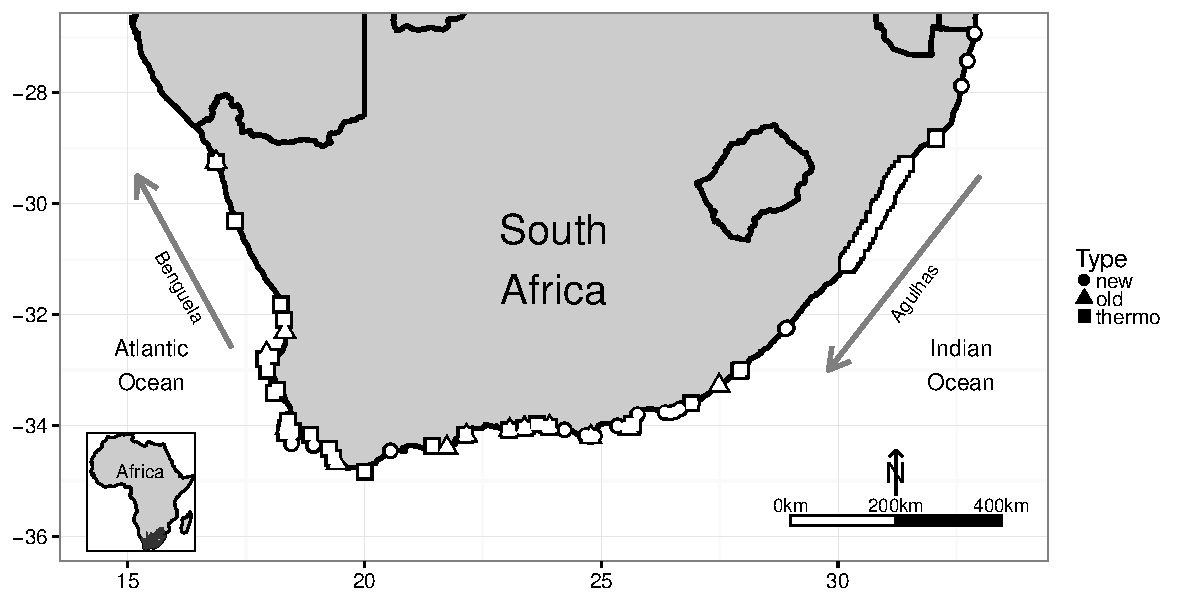
\includegraphics[width=7.5cm]{figure01}
\caption[\small The location of each time series available for use in this study]{The location of each time series available for use in this study.}
\label{figure01}
\end{figure}

\begin{figure}
\centering 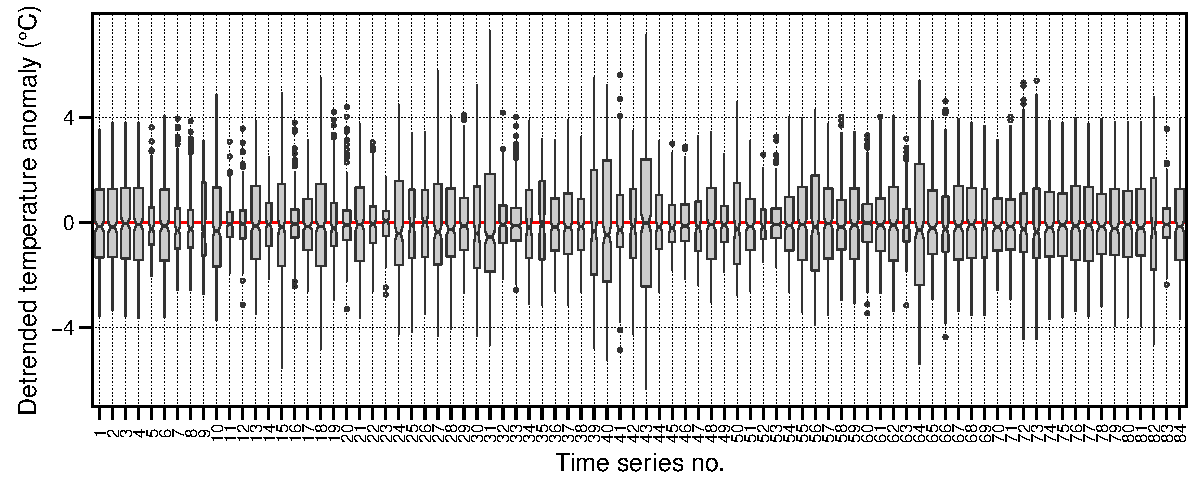
\includegraphics[width=7.5cm]{figure02}
\caption[\small The effect of time series length on the ability of the GLS model to accurately detect the trend added to a time series]{The effect of time series length on the ability of the GLS model to accurately detect the trend added to each time series. The box-and-whisker plots show the first and third quartile as the extremities of the boxes, the median is shown as the horizontal line within each box, and the minima and maxima are indicated by the whiskers. Points indicate the spread of the actual data points and their colors are scaled according to the length of the time seies.}
\label{figure02}
\end{figure}

\begin{figure}
\centering 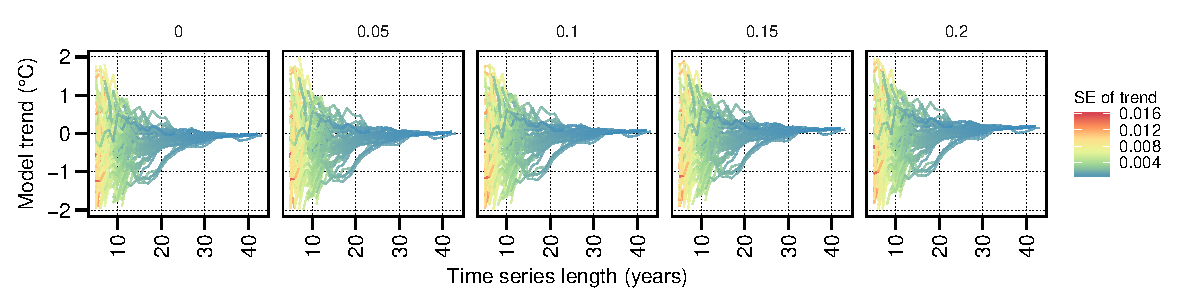
\includegraphics[width=7.5cm]{figure03}
\caption[\small The relationship between time series length and the standard error (SE) of the modelled trend]{The relationship between the length of a time series, the size of the modeled trend and its the standard error (SE). Each individual line shows the modeled trend for one of the 84 sites used in this analysis to which a model was fitted iteratively as the time series length was `grown' from 5 years in length to the maximum duration available for the site.}
\label{figure03}
\end{figure}

\begin{figure}
\centering 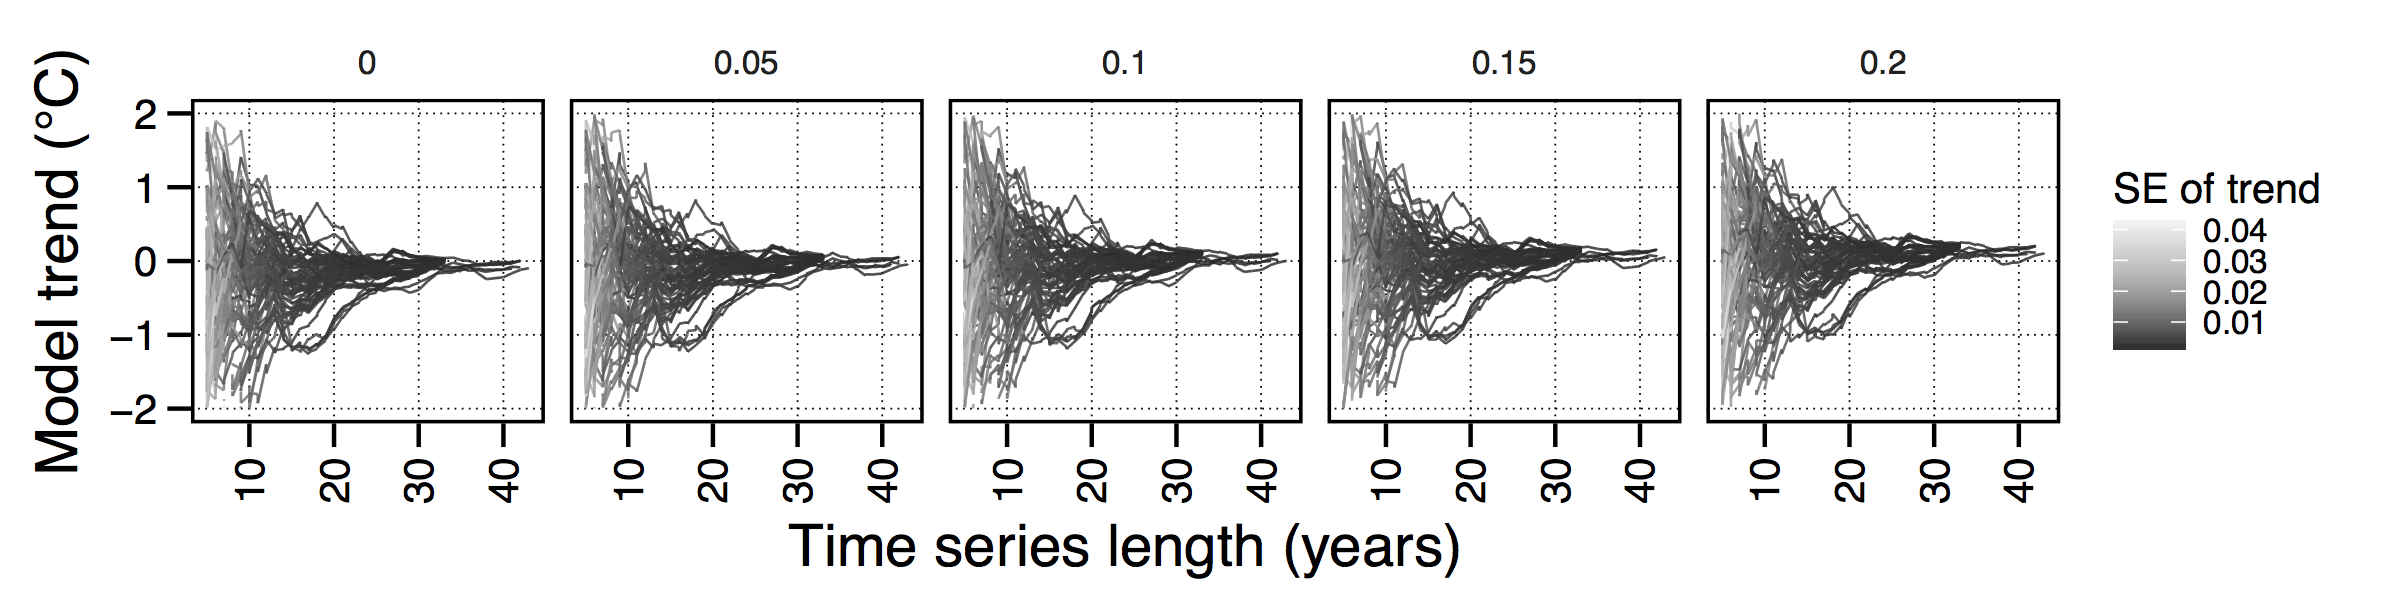
\includegraphics[width=7.5cm]{figure04}
\caption[\small The effect of the natural variation of a time series on the significance of the modelled trend]{The effect of the natural variation of a time series on the significance of the modelled trends estimated by the GLS. The size of the symbols are scaled proportionally to the time series length, with longer time series shown as larger circles.}
\label{figure04}
\end{figure}

\begin{figure}
\centering 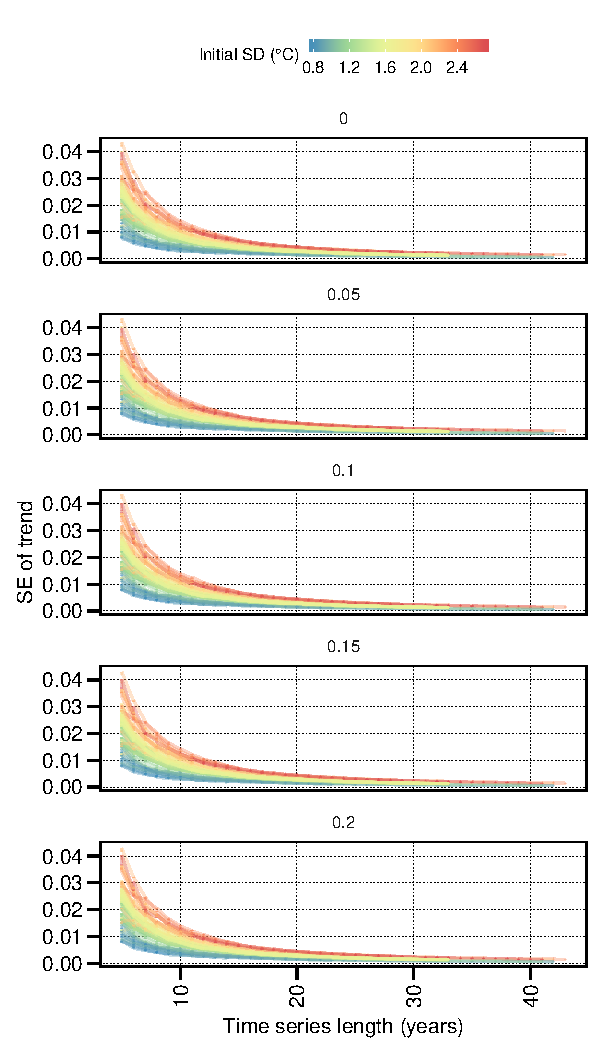
\includegraphics[width=7.5cm]{figure05}
\caption[\small The relationship between the effect of initial SD on the SE of a modelled trend]{The relationship between the effect of the initial SD of a time series on the SE of a modelled trend, controlled for by the length of the time series.}
\label{figure05}
\end{figure}

\begin{figure}
\centering 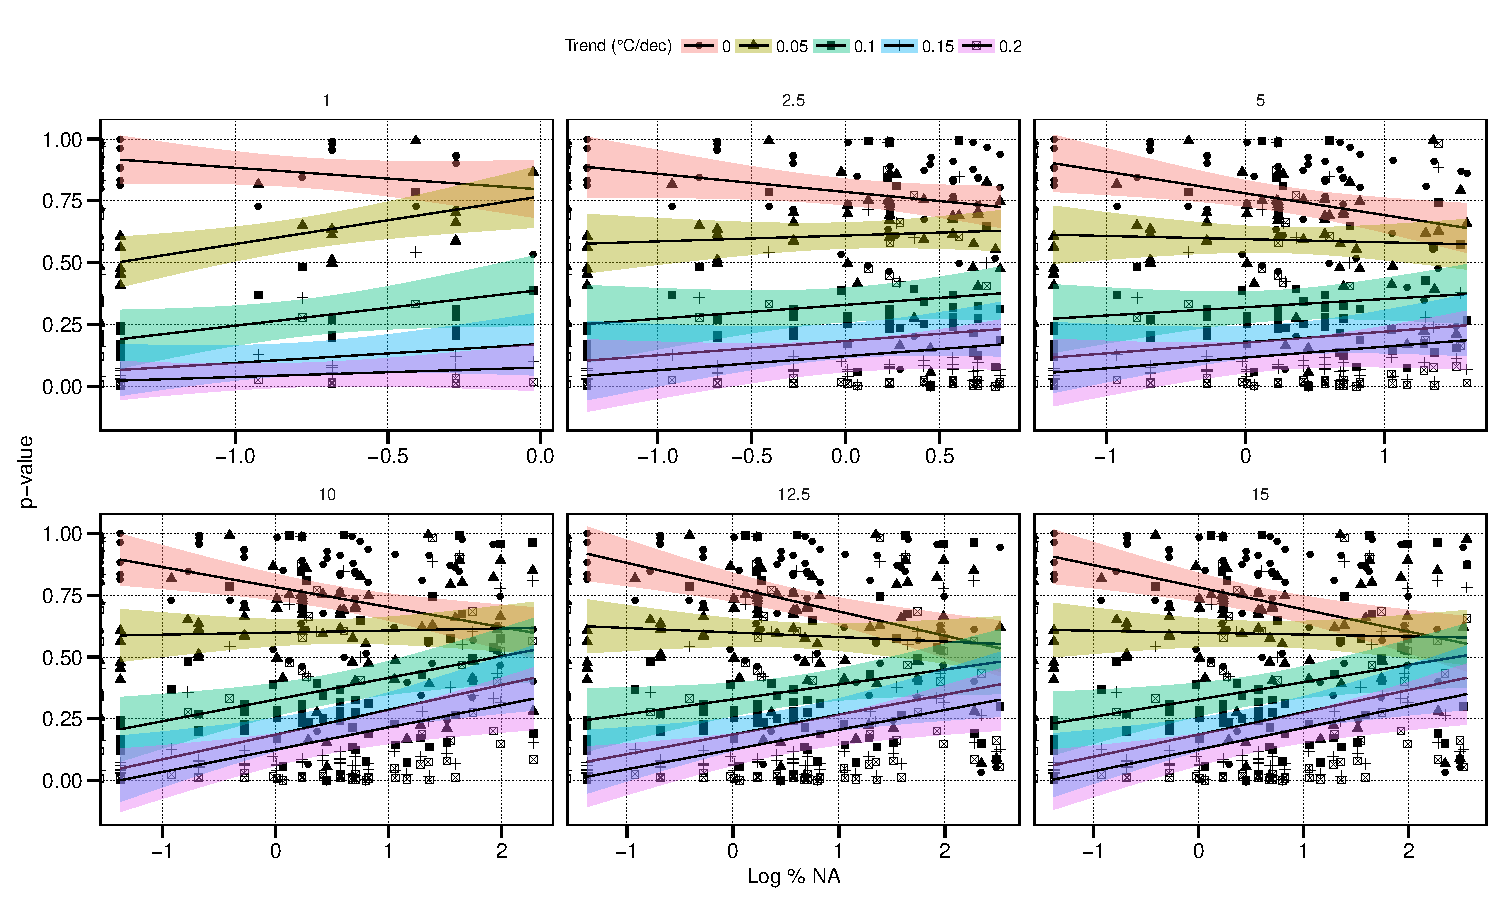
\includegraphics[width=7.5cm]{figure06}
\caption[\small The relationship between \%\texttt{NA} and the significance of a fitted trend]{The relationship between \%\texttt{NA} and the significance of a fitted trend. Each panel shows the effect of an increasingly larger amount of missing values. The the fitted lines and 95\% confidence intervals represent each of the five decadal trends assessed. }
\label{figure06}
\end{figure}

\begin{figure}
\centering 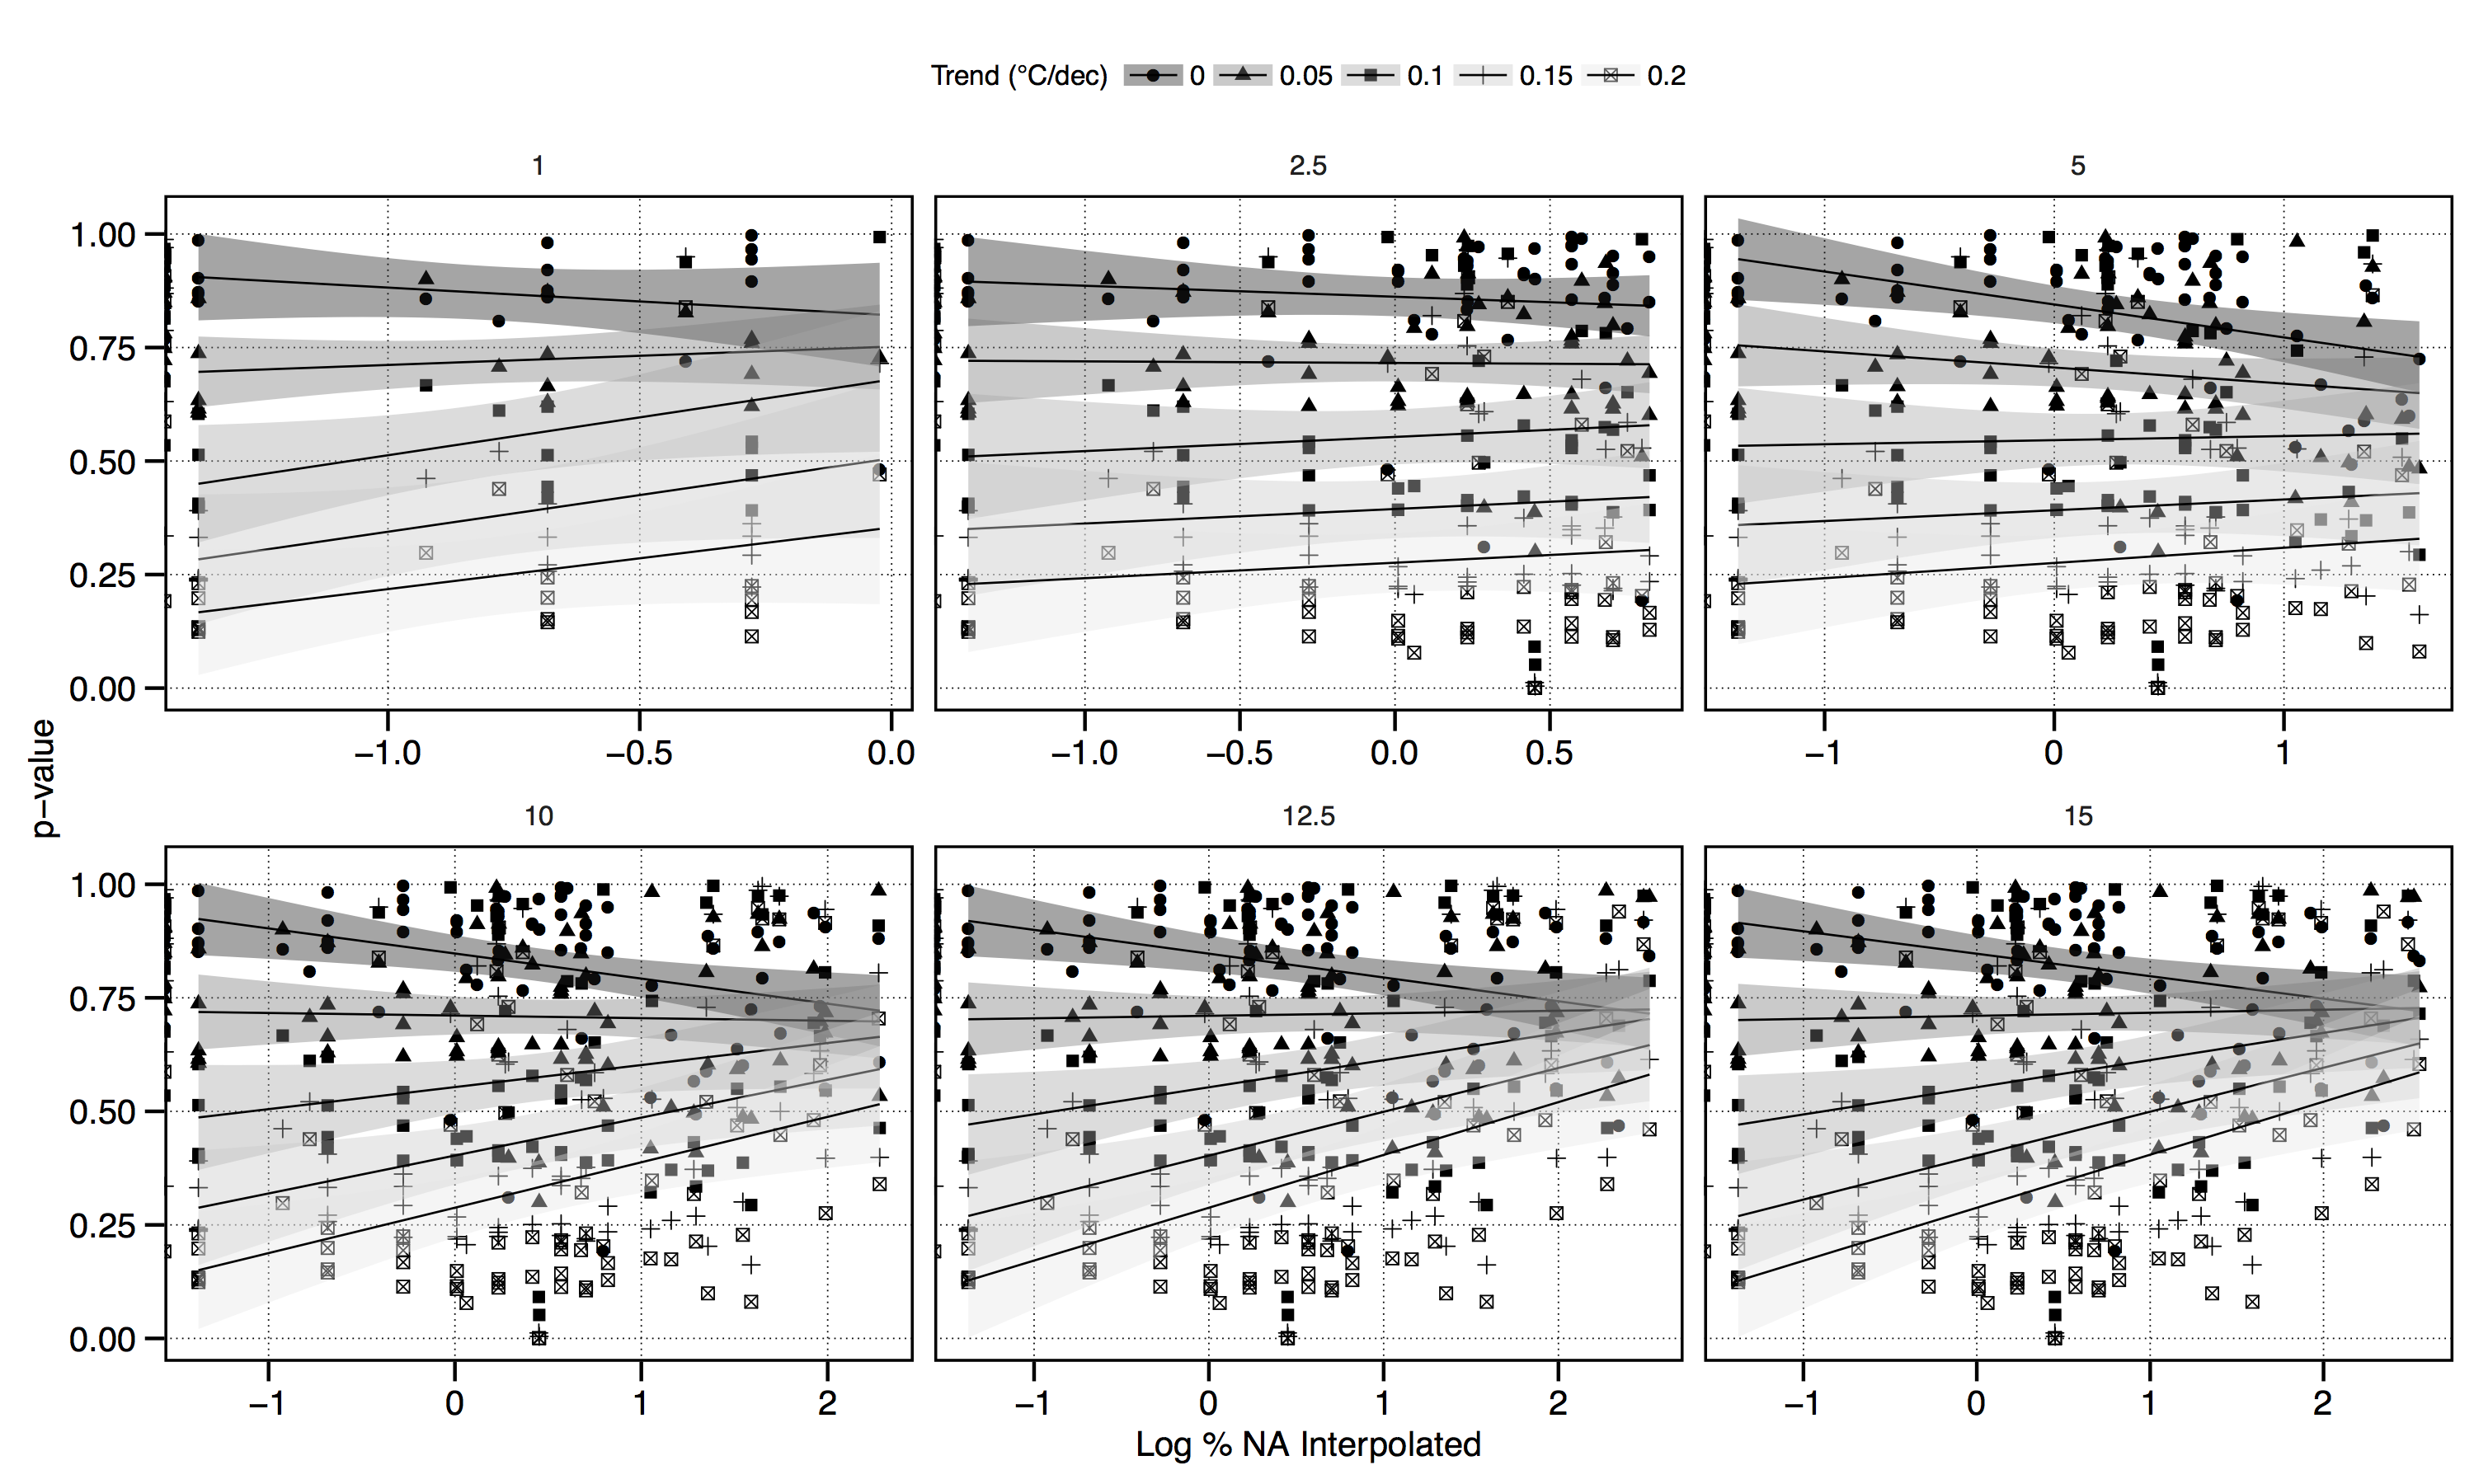
\includegraphics[width=7.5cm]{figure07}
\caption[\small The minimal effect of rounding from]{The minimal effect of rounding from \SI{0.001}{\degreeCelsius} to \SI{0.01}{\degreeCelsius} may be seen in the panel on the right. The panel on the left shows that rounding from a precision of \SI{0.001}{\degreeCelsius} to \SI{0.5}{\degreeCelsius} has a more appreciable effect.}
\label{figure07}
\end{figure}

% RWS - Unsuccesful attempt at adding correct Appendix notation
% \newcommand{\beginsupplement}{%
%         \setcounter{table}{0}
%         \renewcommand{\thetable}{A\arabic{table}}%
%         \setcounter{figure}{0}
%         \renewcommand{\thefigure}{A\arabic{figure}}%
%      }
% \beginsupplement

\begin{figure}
\centering 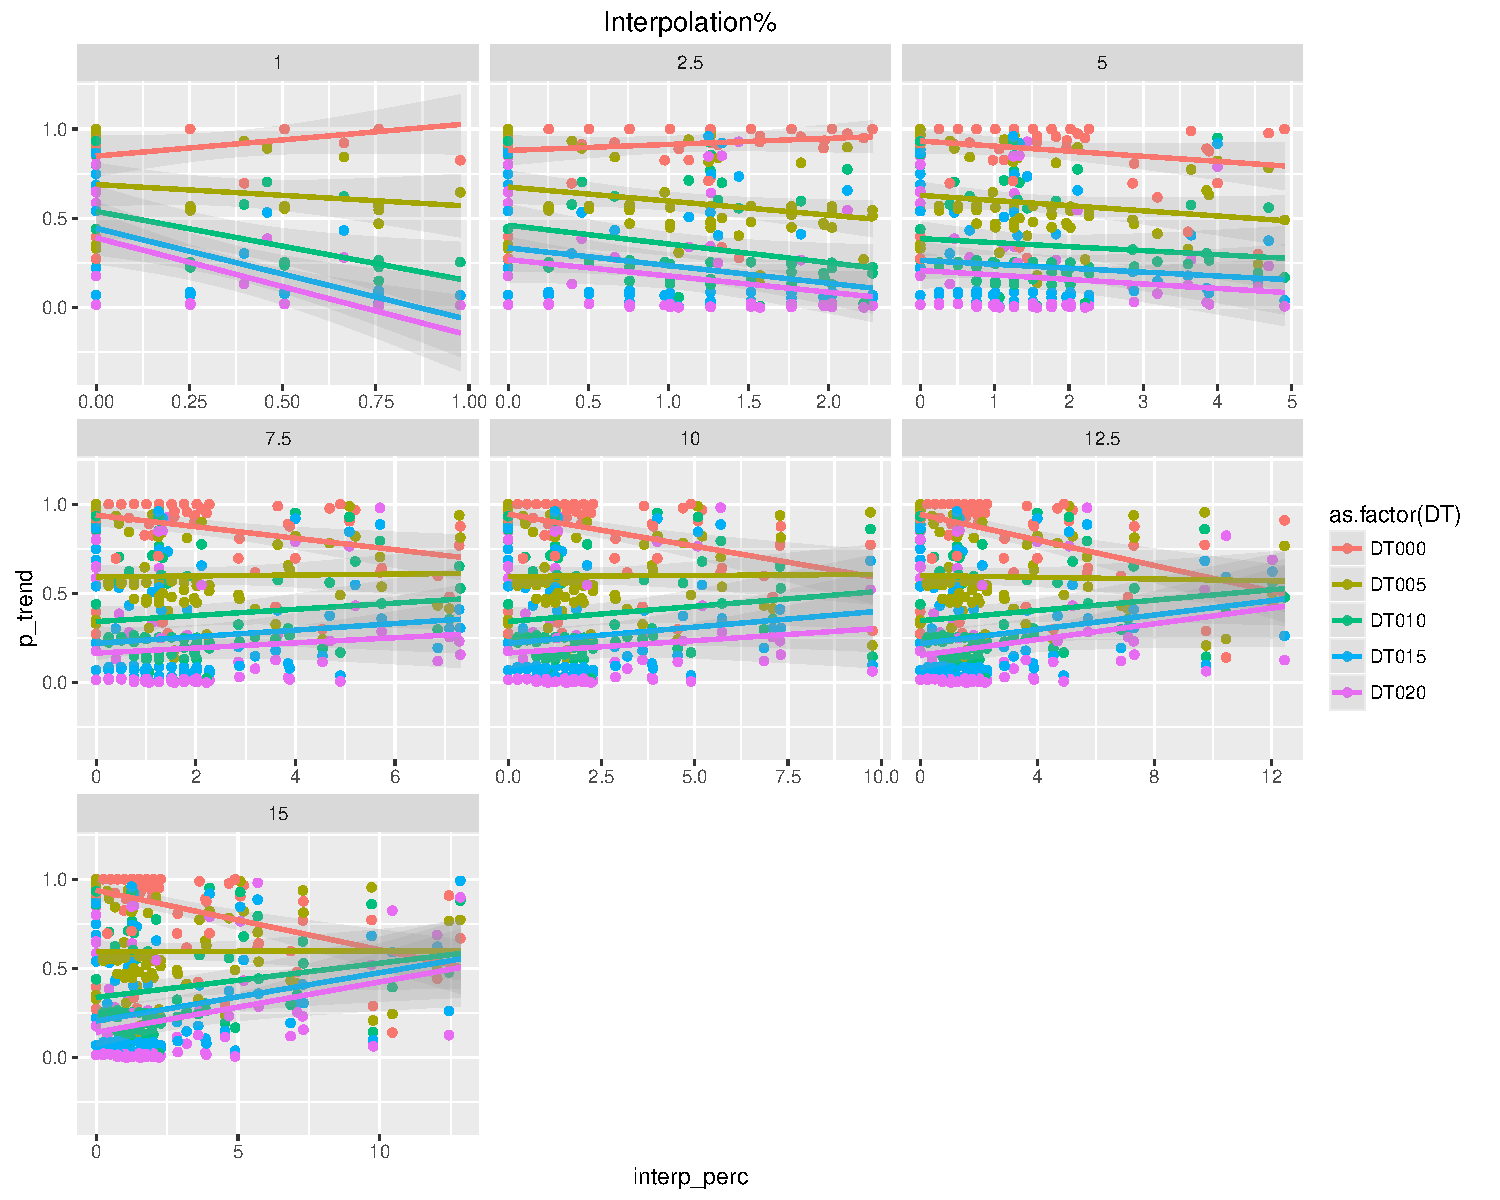
\includegraphics[width=7.5cm]{figureA}
\caption[\small Similar to Figure \ref{figure06}, this figure shows the effect missing data have on]{Similar to Figure \ref{figure06}, this figure shows the effect missing data have on the significance of the slopes detected by GLS however; the missing values in the time series have been filled here via linear interpolation. The effect this has on the significance of the modeled trends is both immediate and dramatic. The behaviour of the quantity of interpolated data also differs from the effect of data left simply as \texttt{NA}. At lower levels of interpolation, missing data actually aid in the fitting of a more significant trend line. This phenomena reverses around 5\%\texttt{NA} when the relationship becomes negative, meaning that as the amount of interpolated data increase, the significance of the fitted trend decrereases.}
\label{figureA}
\end{figure}

\end{document}
